%!TEX root = ../template.tex
%%%%%%%%%%%%%%%%%%%%%%%%%%%%%%%%%%%%%%%%%%%%%%%%%%%%%%%%%%%%%%%%%%%
%% chapter1.tex
%% NOVA thesis document file
%%
%% Chapter with introduction
%%%%%%%%%%%%%%%%%%%%%%%%%%%%%%%%%%%%%%%%%%%%%%%%%%%%%%%%%%%%%%%%%%%
\newcommand{\novathesis}{\emph{novathesis}}
\newcommand{\novathesisclass}{\texttt{novathesis.cls}}


\chapter{Introduction}
\label{cha:introduction}

\begin{quotation}
\begin{flushright}
\itshape
«“Begin at the beginning," the King said, very gravely, \\"and go on till you come to the end: then stop.”»\\
\textbf{- Lewis Carroll, Alice in Wonderland}
\end{flushright}
\end{quotation}

Health is one of the pillars of well-being. Although very precious, health is volatile and subject to constant disturbances imposed by disease and injury. One such type of disturbance is caused by burn injuries. Burn injury still has an expression worldwide as a cause of death and contribute heavily to morbidity and disability.

This work presents a tool concept which results from the combination of different scientific fields, with the goal of improving the treatment of various types of skin wounds, in particular the case of burn injuries.\\

Next, on this chapter, a brief overview of the reality of burn injury and its relation to 3D bioprinting will be presented. Afterwards, a case is made to show that two independent scientific fields can contribute to the development of the tool concept presented by this thesis. The goal of the thesis will be presented, followed by an overview of the proposed system architecture, and culminating on the summary of the document structure.

% ==============================
% = The reality of burn injury =
% ==============================
\section{The reality of burn injury and 3D bioprinting} % (fold)
\label{sec:the_reality_of_burn_injury}

Burn injuries are still a prevalent problem in today's society, claiming the lives of about 17 people worldwide, every hour, according to \gls{who} statistics from 2016 \cite{GHE2016_xls}. Although it represents a small percentage of global death numbers, burn wounds have a significant impact on morbidity and mortality and are considered the worst type of traumatic injury \cite{isbi_guidelines_burn_care}. They also represent a considerable societal cost associated with the expenses for medical care and physical or psychological rehabilitation \cite{Brusselaers_2010_europe_systematic_review}. When not leading to death, they commonly leave the person "with lifelong disabilities and disfigurements, often with resulting stigma and rejection" \cite{who2011_sucess_stories}.\\

Injuries result from "an uncontrolled transfer of energy to the human body in amounts that a body cannot tolerate" \cite{who2011_sucess_stories}. Burn injuries are produced by the transfer of radiation or thermal, electrical and chemical energies to the body. Some examples are direct contact with flames, hot objects or liquids (scalds); exposure to ionising radiation; or contact with high electrical currents, or chemicals \cite{who_unicef2008_burns_chapter}. Burn wounds are typically external wounds inflicted to the skin. Only in some cases like inhalational burns and electric burns the injury is internal and affects something other than the skin.

The skin, the major part of the integumentary system, is the largest organ on the body. It covers the whole surface of the body and has several important functions. It contributes to thermal regulation; works as a protection layer (from UV radiation, microbes, mechanical and thermal offences) for the underlying tissues; acts as a sensitive layer for touch, temperature or pain; allows the excretion and absorption of water and other substances; is a blood reservoir; and synthesises vitamin D \cite{Tortora2009_principles_anatomy_physiology}. 

Concerning its structure (Fig. \ref{fig:skin_structure}), the skin is composed of three layers. The outermost layer is called the epidermis which is a stratified squamous epithelium. It is the main protective barrier. The middle layer is called dermis which is mostly conjunctive tissue.  It is very important because it also contains hair follicles, nerves, sebaceous and sweat glands, blood vessels, and some fat cells. Finally, the innermost layer is the hypodermis. It is mainly adipose and areolar tissues and also contains blood vessels \cite{Tortora2009_principles_anatomy_physiology}.\\

\begin{figure}[htbp]
	\centering
	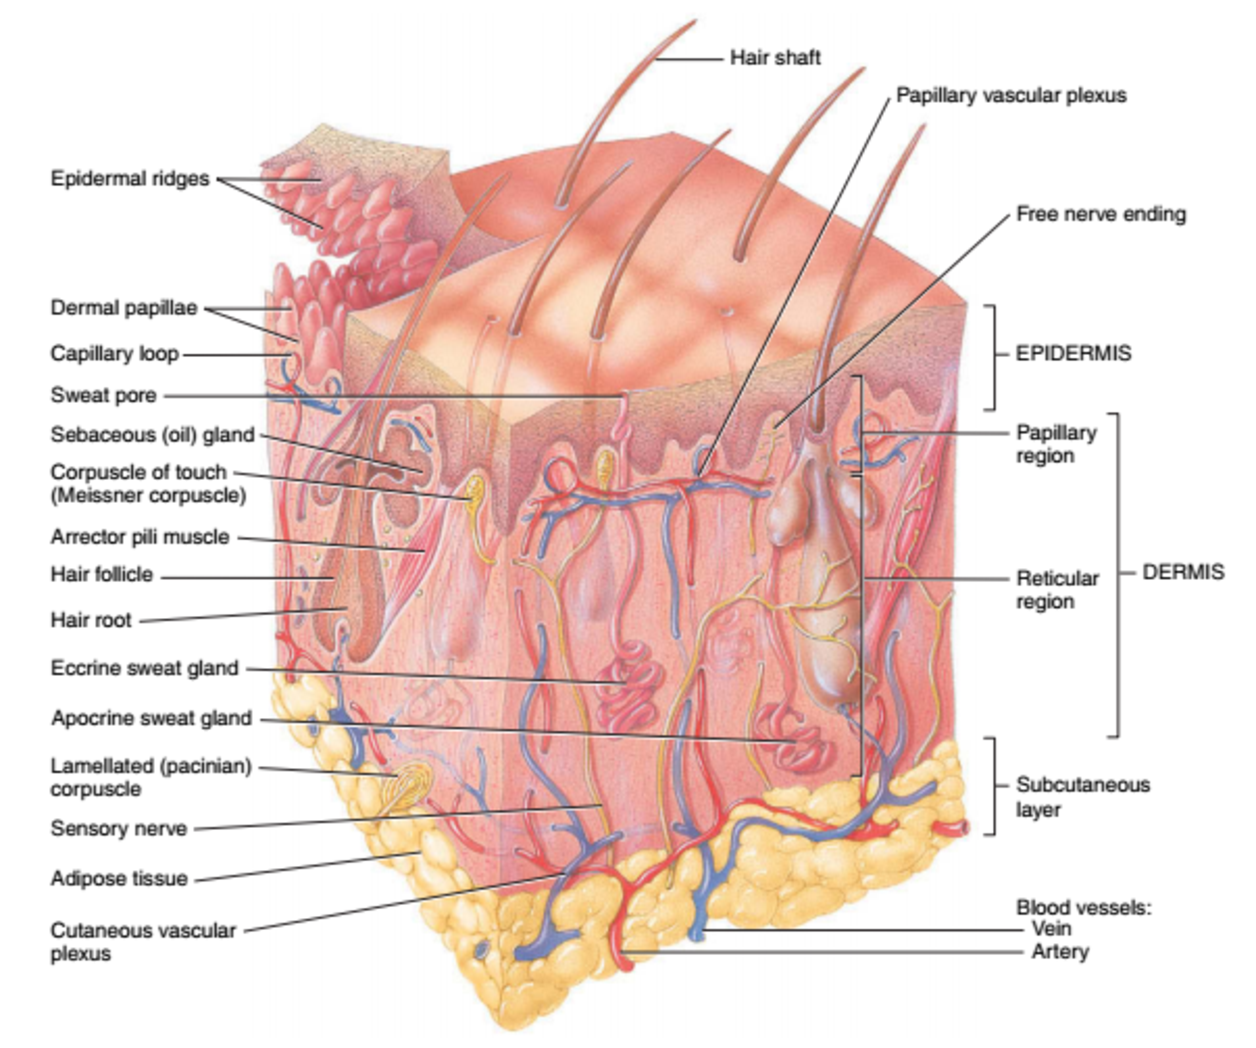
\includegraphics[width=\textwidth]{skin_structure}
	\caption[Sectional view of skin and subcutaneous layer.]{Sectional view of skin and subcutaneous layer. Adapted from \cite{Tortora2009_principles_anatomy_physiology}}
	\label{fig:skin_structure}
\end{figure}

Various criteria are used to classify burn wounds. The mechanism or cause, the extension, and degree or depth, are the most common \cite{who_unicef2008_burns_chapter}. The cause of the wound is related to the energy source involved on the injury formation. The burn extension is clinically referred as the \gls{tbsa} burned, or how much surface area of the skin was burned. The degree or depth is very important because it is directly related to the type of treatment applied. It is separated in three degrees: (a) first-degree, or superficial burns; (b) second-degree, or partial-thickness burns; and (c) third-degree, or full-thickness burns \cite{who_unicef2008_burns_chapter}. 

A first-degree wound only impacts the epidermis (Fig. \ref{fig:burn_wound_degrees}). It takes about a week to heal. Second-degree burns already affect epidermis and dermis (Fig. \ref{fig:burn_wound_degrees}). The healing process takes about 3 to 4 weeks but it still can heal by itself. Hair follicles, sebaceous and sweat glands are generally unaffected, but it loses some of its functions \cite{Tortora2009_principles_anatomy_physiology}. A third-degree burn wound impacts all three layers (Fig. \ref{fig:burn_wound_degrees}). The skin loses most of its functions \cite{Tortora2009_principles_anatomy_physiology} and it generally needs a skin graft to heal properly \cite{who_unicef2008_burns_chapter}. In some cases, a fourth-degree is referred, and it is when the injury crosses all three layers of skin and also affects the underlying tissues like fascia and muscles, or even bone \cite{Vijayavenkataraman2016_stateart_modelling_materials_processing}.

\begin{figure}[htbp]
	\centering
	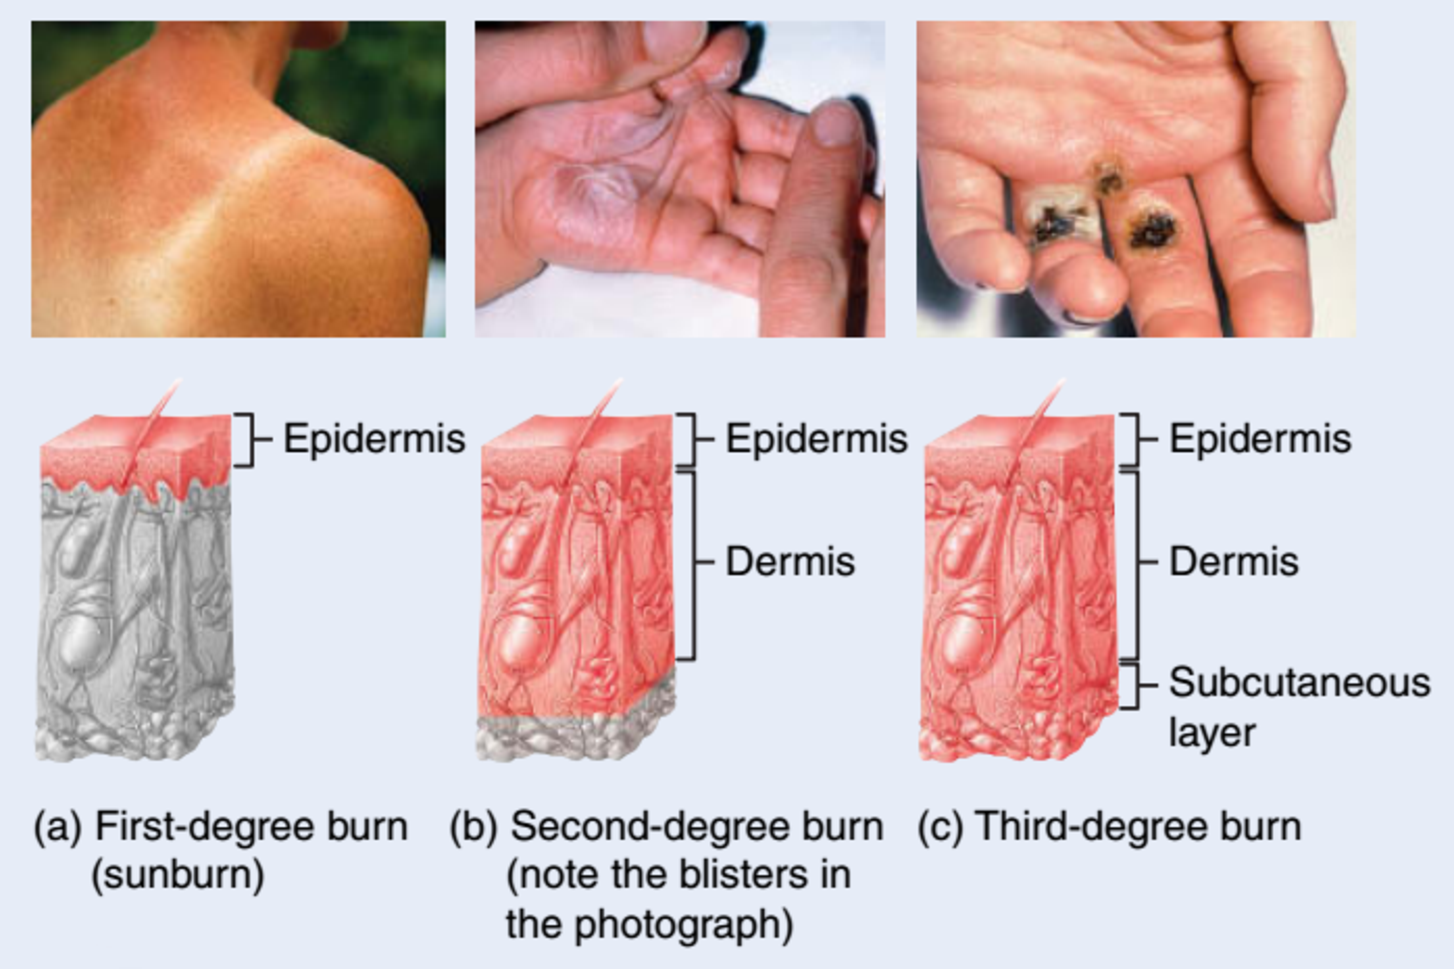
\includegraphics[width=.9\textwidth]{burn_wound_degrees}
	\caption[Burn wound degree and how it affects the skin layers.]{Burn wound degree and how it affects the skin layers. Adapted from \cite{Tortora2009_principles_anatomy_physiology}}
	\label{fig:burn_wound_degrees}
\end{figure}

The \gls{tbsa} and the wound depth have major impact on morbidity and mortality. Larger \gls{tbsa} and deeper wounds directly impact the need of emergency care and hospitalisation, the complexity of the treatment, and the \gls{los} \cite{Santos_2016_burden_burns_portugal, Bartosch_2013_mortality_lengthofstay}. Naturally, this increases the overall costs of treatment, and the burden of the injury. 

In Portugal, a clinical and economical analysis of burn injuries, encompassing a period of 13 years, revealed an average direct cost per year of 13 million Euros, and 6741 Euros per hospitalisation \cite{Santos_2016_burden_burns_portugal}. \gls{is}, which is one type of stroke (the second main cause of death worldwide \cite{GHE2016_xls}), has an average direct cost of hospitalisation of 2215 Euros \cite{Santos_2017_atrial_fibrillation_stroke}. Comparing the hospitalisation costs and the number of associated deaths per year, we can see that burns have a lower number deaths, but cost three times more, on average. This clearly shows the financial impact of burn wound treatment.

Improving the quality of the burn wound care can have direct impact on treatment costs and overall outcome. The aim is to develop a treatment solution that induces rapid healing, without or with minimal scar formation, that significantly reduces the \gls{los}, morbidity and mortality. It should also be cost effective to reduce the financial impact. \\

The standard for treating extensive burn wounds is to use autologous skin grafts. When not possible, allografts or biological and synthetic skin substitutes are used. Skin substitutes help the wound healing process but they are not full skin replacements. 3D bioprinting, a branch of \gls{te}, as brought new perspectives on skin regeneration and healing, and holds promise of significant improvement on burn wound regeneration and scar reduction.

3D Bioprinting is an advanced manufacturing process to fabricate tissue constructs and organs via layer-by-layer deposition of cells, biomaterials and growth-factors, using \gls{cad}, in a repeatable and flexible way \cite{Ng2016_skin_bioprint_reality_fantasy}. This approach to \gls{te} was motivated by the inability of the classical approach to "fabricate complex biomimetic structures [which] results in an over-simplified tissue construct, thus rendering the engineered tissue inaccurate with unrealistic cell microenvironments" \cite{Vijayavenkataraman2018_bioprinting_tissues_organs_regen_med}. Plus, the increasing demand for organs for transplantation, the rise of bans for animal testing, and the need for better in vitro models for drug research and development, as fuelled the development of this technology \cite{Vijayavenkataraman2018_bioprinting_tissues_organs_regen_med}.

The technology has some advantages like the possibility of automation; high precision on cell and material placement, geometrical freedom on the construct shape, the capability to use a wide range of materials, reproducibility, and repeatability \cite{Vijayavenkataraman2018_bioprinting_tissues_organs_regen_med}. However, like all technologies it is not without its limitations. Currently, 3D Bioprinting is not ready for full scale deployment on the healthcare sector. Although it has several reported successes, it is still on its infancy, and has a lot of room for improvement and standardisation \cite{Vijayavenkataraman2018_bioprinting_tissues_organs_regen_med, Datta2018_essential_steps_bioprinting}. 

To 3D bioprint a tissue construct a three stage process is followed. It starts with pre-bioprinting, followed by the bioprinting stage and ends with post-bioprinting \cite{Datta2018_essential_steps_bioprinting, Vijayavenkataraman2018_bioprinting_tissues_organs_regen_med}. All three stages have their limitations and a concerted effort of the whole community is needed to take this technology from bench to bedside. Some of the improvements needed on the bioprinting stage are a higher number of degrees of freedom of the bioprinting system; higher printing speeds without compromising the cells viability and construct shape; and increased automation of the printing process \cite{Ozbolat2017_evaluation_bioprinter_tech, Datta2018_essential_steps_bioprinting}. Collaborative robotics and computer vision can help solve these limitations.

% section the_reality_of_burn_injury (end)

% ===========================================================
% = Development of complementary technologies and practices =
% ===========================================================
\section{Development of complementary technologies and practices} % (fold)
\label{sec:development_of_complementary_technologies_and_practices}

In parallel with the development of 3D bioprinting, other areas of science and technology have evolved which can contribute to its improvement. Here, two areas are emphasised because they complement each other to open new roads for automated in situ bioprinting. They are \textbf{collaborative robotics} and \textbf{computer vision}.

% = Collaborative Robotics =
\subsection{Collaborative Robotics} % (fold)
\label{subsec:collaborative_robotics}

The use of robotics revolutionised many industries, from cars to food. Today, most industries use some kind of robotic tool to automate procedures and increase efficiency. One of the problems associated with industrial robotic manipulators is their inability to work alongside humans. Because of this security concern, the use of robotic manipulators on other settings was not seen as a good option.

This limitation, along with developments on motor technology and electronics, motivated the development of a new breed of robotic manipulators and control architectures, and culminated on a new branch of robotics called collaborative robotics. 

Collaborative manipulators are smaller and lighter than their industrial counterparts. They use electric actuators which are cleaner, less noisy and less bulky, contributing to smaller robots and a cleaner working environment. They can also be used in more cluttered spaces, common in many human workspaces.

A key factor on their success is the control architectures used. Using more accurate dynamic models, they can take into consideration interaction forces of the robot with the environment. This allows to control the robot compliance and make it apparently soft when interacting with a human \cite{Bloss2016_collaborative_robotics_improvements}.

Robots also have impacted the medical field. The first use of a robot in this field was in the late 1980s when a PUMA robot was used to orient a needle for brain biopsy with computer-tomography (CT) guidance \cite{Kwoh1988_puma_brain_surgery}. From there, other systems were developed for orthopaedic surgery, laparoscopic surgery, and others. In 2000, the robot Da Vinci from Intuitive Surgical was the first FDA approved surgical robotic system \cite{FoodAndDrugAdministration2000_fda_approves_davinci}.

New research in medical systems using collaborative robotics has emerged. Some examples are: robotic assisted tele-echography \cite{Santos2018_computed_torque_control_robotic_assisted_tele_ecography}; collaborative robotics for cancer staging biopsies \cite{Esposito2016_collaborative_robotics_cancer_staging_biopsies}; and COVID-19 throat swabing robot \cite{Dalgaard2020_covid19_swabing_robot}.

Collaborative robotics, with new manipulators and control architectures, brings another card to the table by permitting the coexistence of humans and robots on the same workspace, and most importantly, allowing human-robot collaboration.

% subsection collaborative_robotics (end)

% = Computer Vision =
\subsection{Computer Vision} % (fold)
\label{subsec:computer_vision}

Computer Vision and Image Processing are two important fields of computer science. The goal of image processing is to generate new images by changing some of the initial image's properties or information. Computer vision tries to extract information from an image just like a human would by using machine learning techniques on top of image processing.

Computer vision algorithms have been used in many different scientific and engineering fields. Two important examples are its use in medicine and robotics.

Computer vision is a fundamental branch of robotics. Many robotic systems do not have vision capabilities, but when autonomy is important, vision is a common sensory option. From mobile to humanoid robots, vision adds a human-like skill to analyse the environment. Robotics has contributed positively for the development of computer vision. The computer vision algorithms within the robotic realm have been used for inspection, for the detection of objects, people and faces \cite{Fang2018_facial_detection}, and more.

In medicine, computer vision also has an important role that has been increasing with time. This computer ability has been used for things like cell counting \cite{He2019_cell_counting} to culture inspection. New machine learning algorithms have been used to detect cancer in histological slides \cite{Araujo2017_classification_breast_cancer_histology}, for example. An important example on the realm of burn injury is the use of computer vision to segment burn wounds and classify the \gls{tbsa} \cite{Wantanajittikul2012_automatic_segmentation_degree_identification_burn_wounds}. Not to mention all the branches of medical imaging that depend on it to extract vital diagnostics data from medical images.

Computer Vision is a mature scientific branch of computer science that has produced considerable advances in robotics and medicine. Its tools and algorithms will continue to improve the automation capabilities of the systems where they are used.

% subsection computer_vision (end)

% section development_of_complementary_technologies_and_practices (end)

% =========
% = Goals =
% =========
\section{Goals} % (fold)
\label{sec:goals}

By combining the capabilities of 3D bioprinting, collaborative robotics and computer vision, the present thesis proposes to develop a semi-autonomous 3D positioning system for bioprinting skin tissue construct directly on burn wounds. The main goal of the system is to detect burn wounds, devise a printing path, and be able to travel through that path at a certain speed while dispensing bioink. This goal encompasses several specific goals, to mention:

\begin{enumerate}
    \item Detection and segmentation of burn wounds;
    \item Definition of wound area, perimeter and localisation;
    \item Path and Trajectory planning;
    \item Robot manipulator control for trajectory execution;
    \item Print head control for bioink dispensing.
\end{enumerate}

The broader goals of this work are to show that using a robotic arm with more than 3 \gls{dof} is a valid option for in situ bioprinting; and using a vision system opens the possibility for printing automation. On the bigger picture of medical robotics this work intends to prove that there exists other valid use cases for the use of robotics in surgery and treatment.

% section goals

% ========================================
% = Proposed System Architecture Summary =
% ========================================
\section{Proposed system architecture summary} % (fold)
\label{sec:proposed_system_architecture_summary}

The chosen system architecture aims to solve some limitations of the current 3D bioprinting systems. It consists of three main components: a robotic manipulator that works as a 3D positioning system; a vision system, composed by a stereo camera attached to the manipulator end-effector, to detect burn wounds and contribute to visual servoing; and a bioprinting end-effector system to carry out the bioprinting itself (Fig. \ref{fig:system_architecture_intro}).

\begin{figure}[htbp]
	\centering
	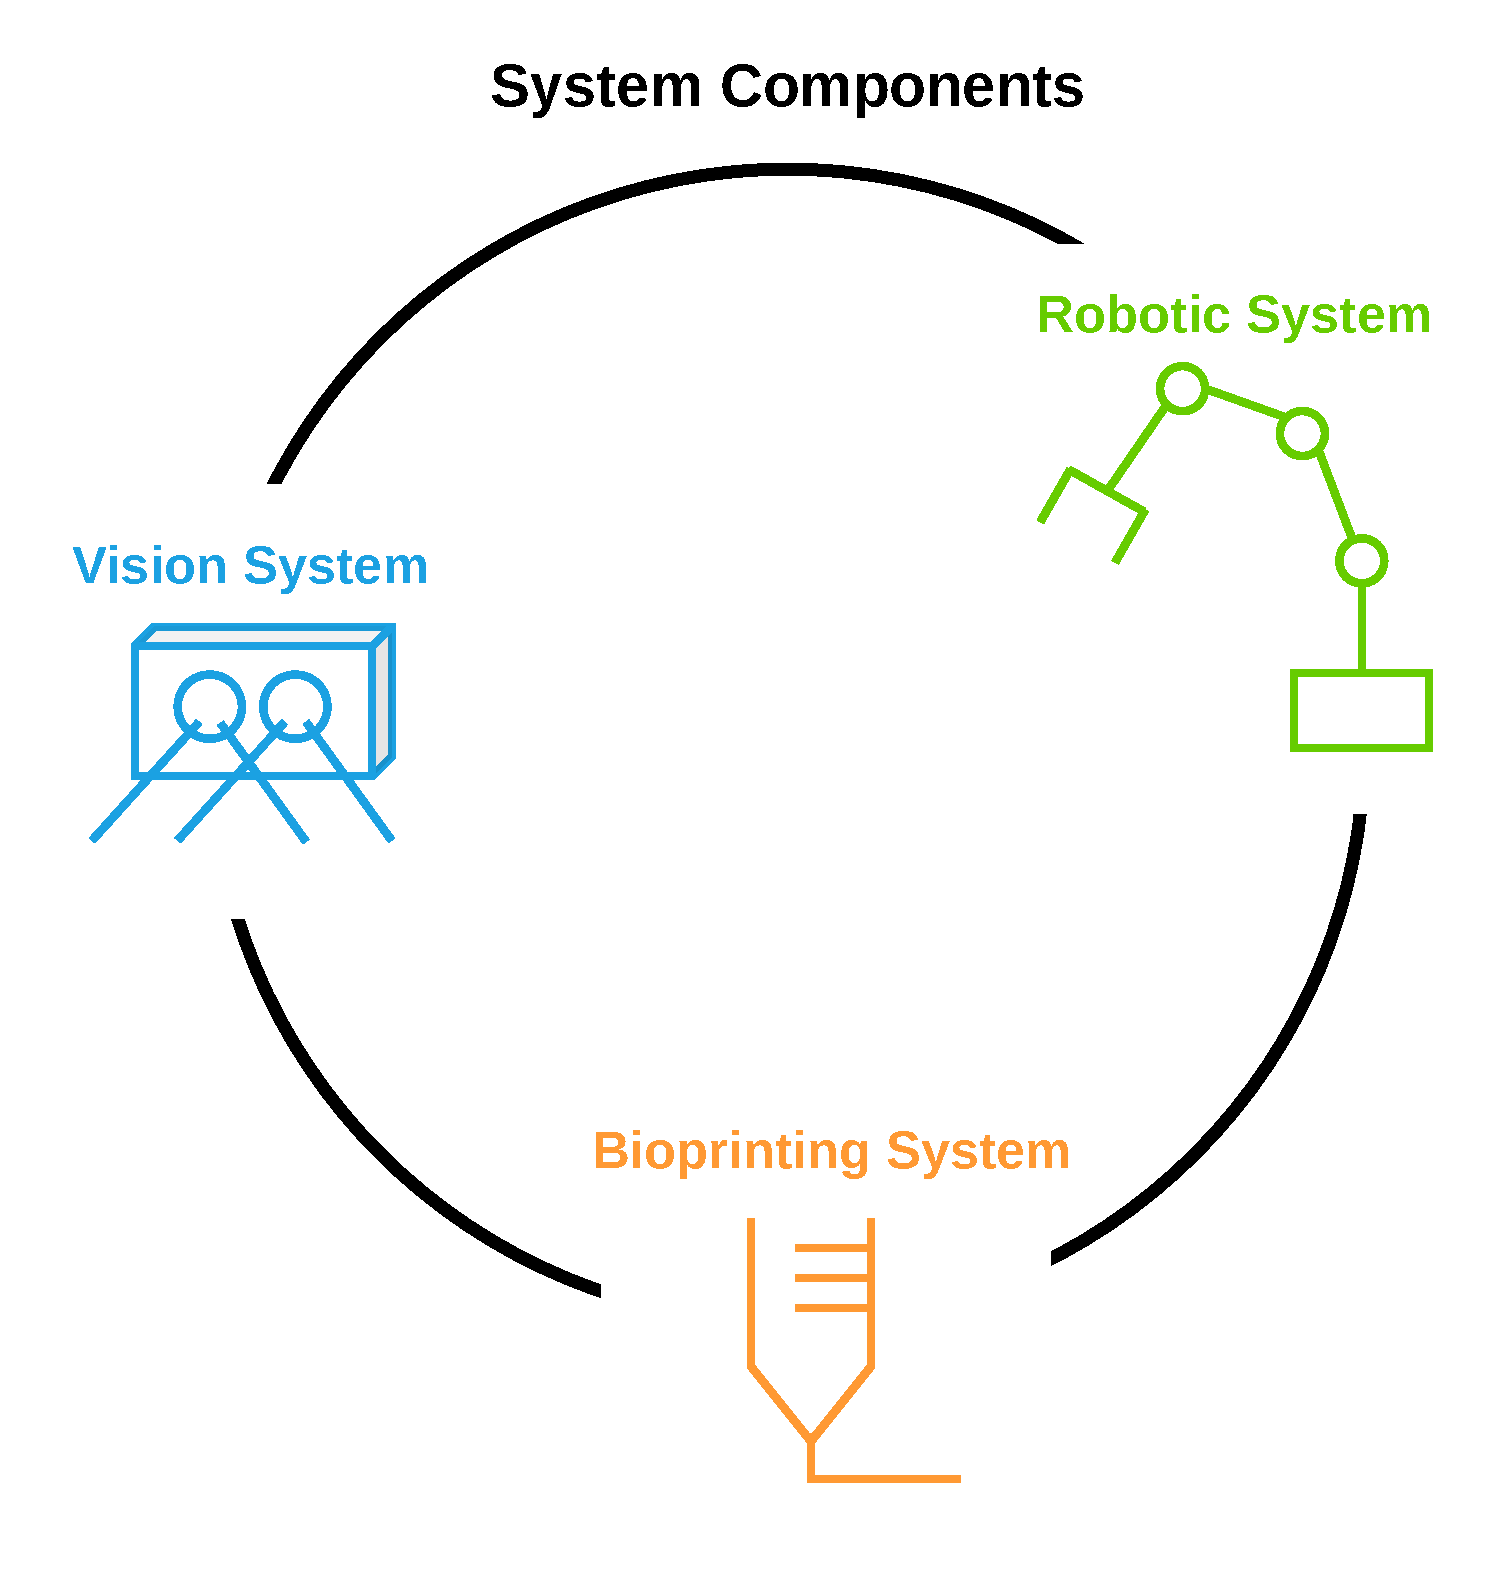
\includegraphics[width=.5\textwidth]{system_architecture_components_intro}
	\hspace{0.1in}
	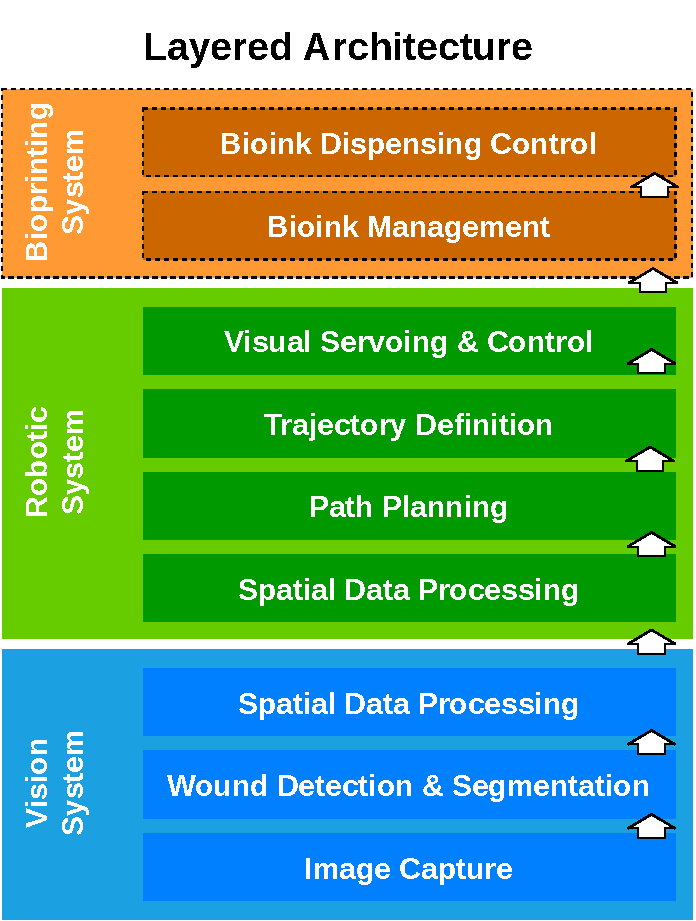
\includegraphics[width=.45\textwidth]{system_architecture_layers_intro}
	\caption[System architecture main components and functional layers.]{System architecture main components (left) and functional layers (right).}
	\label{fig:system_architecture_intro}
\end{figure}

The use of a robotic manipulator brings more \gls{dof} facilitating the bioprinting in non-planar surfaces. Using a camera increases the autonomy of the bioprinting process. The combination of both systems facilitates the 3D bioprinting to be done in situ.

A layered structure is used to describe the system's functional architecture. Composed by nine layers (Fig. \ref{fig:system_architecture_intro}), it aims to organise the system into independent modules that communicate between adjacent layers.

On chapter \ref{cha:system_architecture}, the system architecture will be described in more detail.

% section proposed_system_architecture

% ======================
% = Document structure =
% ======================
\section{Document structure}
\label{sec:document_structure}

The document structure followed aims to guide the reader from the need of the proposed system, to its implementation, and ending on the results obtained and future needs. The thesis is organised into nine interdependent, but self-contained, chapters:

\begin{enumerate}
    \item \textbf{Introduction}, presents the biomedical application context of the proposed tool system, which is the reality of burn injury and 3D bioprinting. It is followed by a summary of two different scientific fields that contribute for the development of the proposed tool. Afterwards, the goal of the thesis and a summary of the proposed system architecture are presented. It ends with the description of the thesis document's structure.
    
    \item \textbf{Theoretical Concepts}, introduces the fundamental concepts of this thesis. It focuses on concepts of 3D bioprinting, robotic control and computer vision. 
    
    \item \textbf{Literature Review}, consists on an analysis of the current literature related with 3D bioprinting using robotic manipulators, with or without vision systems.
    
    \item \textbf{System Architecture}, is a full description of the proposed system architecture. It starts with a description of the system requirements. Subsequently, the robotic, vision, and bioprinting systems are introduced. Finally, the system's functionality and interaction layers are described in detail.
    
    \item \textbf{Robotic System}, starts with a main overview of the robotic system. It describes the robot operation and robot kinematic and dynamic characteristics. It ends with the integration of the robot with \gls{ros} and Gazebo simulation environment.
    
    \item \textbf{Vision System}, describes the camera system used and the way it interfaces with the robot manipulator. It also describes the integration with \gls{ros} and Gazebo.
    
    \item \textbf{Control Architectures}, discusses the architecture used for robot positioning.
    
    \item \textbf{System Validation}, is where all the test procedures are documented and results presented. It ends with a discussion of the results.
    
    \item \textbf{Conclusions}, presents the main conclusions of the thesis, and proposes future work.
\end{enumerate}

The document also has appendixes and annexes that complement the main body of text present on the previous chapters.

% section document_structure